% -- LaTeX rewrite of main.typ, using the OUP template and matching the structure and content --

\documentclass[unnumsec,webpdf,contemporary,large]{oup-authoring-template}
\usepackage{booktabs}
\usepackage{placeins}
\usepackage{float}

\theoremstyle{thmstyleone}%
\newtheorem{theorem}{Theorem}%
\newtheorem{proposition}[theorem]{Proposition}%
\theoremstyle{thmstyletwo}%
\newtheorem{example}{Example}%
\newtheorem{remark}{Remark}%
\theoremstyle{thmstylethree}%
\newtheorem{definition}{Definition}

\begin{document}

\journaltitle{Oxford University Press.}
\copyrightyear{2025}
\appnotes{Paper}

\firstpage{1}
\setlength{\parindent}{0pt}
\setlength{\parskip}{0em}

\title[Assessing AlphaFold3 on PLA]{Assessing the Reliability of AlphaFold3 Predictions for Protein-Ligand Affinity Prediction via Sfcnn}

\author[1]{Guo Yu}
\author[1]{Yiming Wu}
\author[1]{Yiyang Tan}

\authormark{Guo Yu et al.}

\address[1]{\orgdiv{School of Information Science and Technology}, 
\orgname{ShanghaiTech University}, 
\orgaddress{\street{393 Middle Huaxia Road}, \postcode{201210}, \state{Shanghai}, \country{China}}}

\abstract{
This study systematically evaluates the reliability of AlphaFold3 
(AF3)-predicted protein structures for protein-ligand affinity (PLA) 
prediction tasks. The Sfcnn model, a 3D convolutional neural network 
(CNN) for PLA prediction, was reproduced using PyTorch,
its performance was validated on the PDBbind v2019 refined set 
for training and the CASF-2016 core set for testing. Subsequently, 
AF3-derived protein structures from the CASF-2016 core set were 
assessed and compared to experimentally determined structures 
using Sfcnn scores to determine the suitability of AF3 predictions 
in PLA applications.
}
\keywords{AlphaFold3, protein-ligand affinity, CNN scoring function, CASF-2016}

\maketitle

\section{Introduction}
\vspace{0.5em}
\subsection{Background}
AlphaFold3 (AF3), DeepMind's latest AlphaFold model, predicts protein and protein–ligand structures with high accuracy. It extends AlphaFold2 by adding explicit ligand modeling, enhanced multimer assembly support, and optimized multiple sequence alignments (MSAs) via deep neural networks trained on extensive sequence and structural data~\cite{AF3}.

Sfcnn is a 3D convolutional neural network-based scoring function introduced by Wang et al.~\cite{Sfcnn} in 2022, designed to provide accurate and reliable predictions of binding affinities for protein-ligand complexes.
\vspace{0.5em}
\subsection{Objective}
The primary objective of this study is to evaluate the reliability of AlphaFold3-predicted protein-ligand complex structures for protein-ligand affinity (PLA) prediction. 
Using the Chai-1 server for AF3 structure generation, we utilized its support for custom ligands and robust MSA construction. 
The resulting AF3 structures are assessed with the reproduced Sfcnn model, and predicted affinities are compared to those from experimentally determined structures. 
This enables a direct evaluation of AF3's suitability for PLA prediction and highlights its current strengths and limitations.

\section{Materials and Methods}
\vspace{0.5em}
\subsection{Datasets}
The Sfcnn network was trained using protein-ligand complexes from the PDBbind v2019 refined set\cite{Wang2005PDBbind}, which includes experimentally determined binding affinities (pKa values). The model was evaluated on the CASF-2016~\cite{su2018comparative} core set, comprising 285 protein-ligand complexes. To prevent data leakage, 266 overlapping protein complexes between the training and test sets were excluded, resulting in 4,852 unique training complexes.

\subsection{Data Augmentation}
To increase the effective size of the training set, each protein-ligand complex was randomly rotated nine times using random rotation matrices, yielding ten variants per complex. All variants share the same PLA score, resulting in a total of 48,520 training samples.

\subsection{Featurization}
Protein-ligand complexes are represented as 3D grids of size $20 \times 20 \times 20$, with each grid cell encoded as a one-hot vector of length 28. This vector comprises 14 protein atom types\footnote{\url{https://bmcbioinformatics.biomedcentral.com/articles/10.1186/s12859-022-04762-3}} and 14 ligand atom types. The resulting training tensor has shape $(48520, 20, 20, 20, 28)$.

\begin{figure}[H]
    \centering
    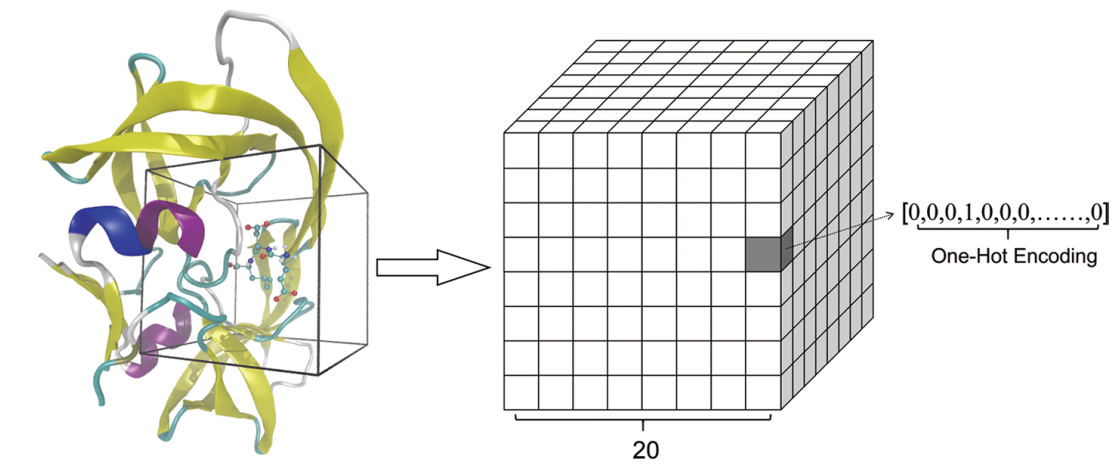
\includegraphics[width=0.5\textwidth]{images/one_hot.png}
    \caption{Featurization of protein-ligand complexes. Example shown: PDB ID 1a30. Resolution is $20 \times 20 \times20$ with 28 atom types.}
    \label{fig:onehot}
\end{figure}

\section{Sfcnn Network Architecture and Implementation}

\subsection{Architecture}
The original Sfcnn publication describes four network architectures and three featurization strategies. The architecture depicted in Figure~\ref{fig:CNN}, combined with the aforementioned featurization, achieved optimal validation performance.

\begin{figure}[H]
    \centering
    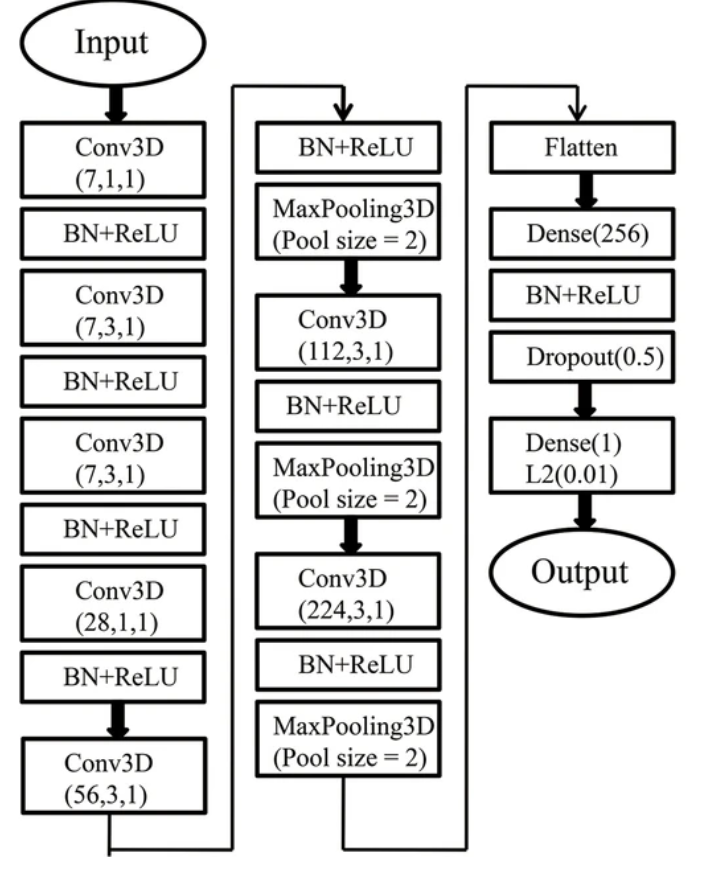
\includegraphics[width=0.35\textwidth]{images/CNN.png}
    \caption{Final CNN architecture for the Sfcnn network.}
    \label{fig:CNN}
\end{figure}

This architecture employs 3D convolutional layers with batch normalization and ReLU activation. L2 regularization is applied to the output layer to mitigate overfitting and enhance generalization.

\subsection{Implementation Details}
The PyTorch implementation closely mirrors the original TensorFlow version, with two key differences:
\begin{enumerate}
    \item Due to PyTorch's \texttt{Conv3D} API, input tensors are permuted to shape (batch\_size, 28, 20, 20, 20).
    \item PyTorch lacks a direct L2 regularization API; instead, weight decay is applied to the final fully connected layer to approximate this effect.
\end{enumerate}

\subsection{Data Storage}
The original Sfcnn implementation stored data as concatenated arrays in a single \texttt{.pkl} (pickle) file, requiring all data to reside in memory, which is impractical for extremely large datasets. The HDF5 format (\texttt{.h5}) via \texttt{h5py} was adopted for incremental writing and efficient storage. The resulting training grid occupies 40.1 GiB.

\subsection{Training Procedure}
Training and validation sets are partitioned using a 7-fold cross-validation 
approach on the entire training dataset of 48,520 samples. The dataset was randomly 
shuffled and divided into 7 folds, 
maintaining consistent train-validation splits across experiments. For each fold, 
approximately 85\% of the data (around 41,242 samples) is used for 
training and 15\% (around 7,278 samples) for validation. 
The test set comprises 285 samples. 
The cross-validation framework enables comprehensive evaluation 
of model stability and generalization capability while providing 
statistical confidence intervals for performance metrics.

Note that the original hyperparameters did not yield convergence 
in our PyTorch experiments. Both sets of hyperparameters are summarized below.

\begin{table}[H]
\centering
\caption{Original and Reproduced Hyperparameters}
\label{tab:hyperparams}
\begin{tabular}{lcc}
\toprule
Parameter & Original & Reproduced \\
\midrule
Learning rate & 0.004 & 0.00068 \\
Batch size & 64 & 32 \\
Dropout rate & 0.5 & 0.15 \\
L2 regularization / FC weight decay & 0.01 & 0.01 \\
Epochs & 200 & 150 \\
Train/validation split & 85\%/15\% & 85\%/15\% \\
\bottomrule
\end{tabular}
\end{table}

\section{Reproduced Results}
\label{sec:ReproducedResults}

\subsection{Evaluation Metrics}
Sfcnn performance is evaluated using the following metrics:

\begin{align*}
\mathrm{RMSE} &= \sqrt{\frac{1}{N} \sum_{i=1}^{N} (y_{\text{predict}} - y_{\text{true}})^2} \\
\mathrm{MAE} &= \frac{1}{N} \sum_{i=1}^{N} |y_{\text{predict}} - y_{\text{true}}| \\
\mathrm{SD} &= \sqrt{\frac{1}{N-1} \sum_{i=1}^{N} ((a y_{\text{predict}} + b) - y_{\text{true}})^2} \\
\mathrm{R} &= \frac{\mathbb{E}[(y_{\text{predict}} - \mu_{y_{\text{predict}}})(y_{\text{true}} - \mu_{y_{\text{true}}})]}{\sigma_{y_{\text{predict}}} \sigma_{y_{\text{true}}}}
\end{align*}

where $a$ and $b$ are the slope and intercept of the linear regression between predicted and measured values, $\mathbb{E}[\cdot]$ denotes expectation, and $\mu$ and $\sigma$ represent means and standard deviations, respectively.

\begin{table}[H]
\centering
\caption{Highest Performance Metrics on CASF-2016 Core Set}
\label{tab:metrics}
\begin{tabular}{lcc}
\toprule
Metric & Reproduced Sfcnn & Original Sfcnn \\
\midrule
Pearson R & 0.7678 & 0.7928 \\
RMSE & 1.4647 & 1.3263 \\
MAE & 1.1633 & 1.0277 \\
SD & 1.3928 & 1.3252 \\
\bottomrule
\end{tabular}
\end{table}

The 7-fold cross-validation yielded a mean test Pearson correlation of $0.7375 \pm 0.0145$ and
the highest Pearson correlation of $0.7678$ on the CASF-2016 core set, as shown in Table~\ref{tab:metrics},
demonstrating consistent model performance across different data partitions and confirming the reliability of our reproduced implementation.


\begin{figure}[H]
    \centering
    \begin{minipage}{0.4\textwidth}
        \centering
        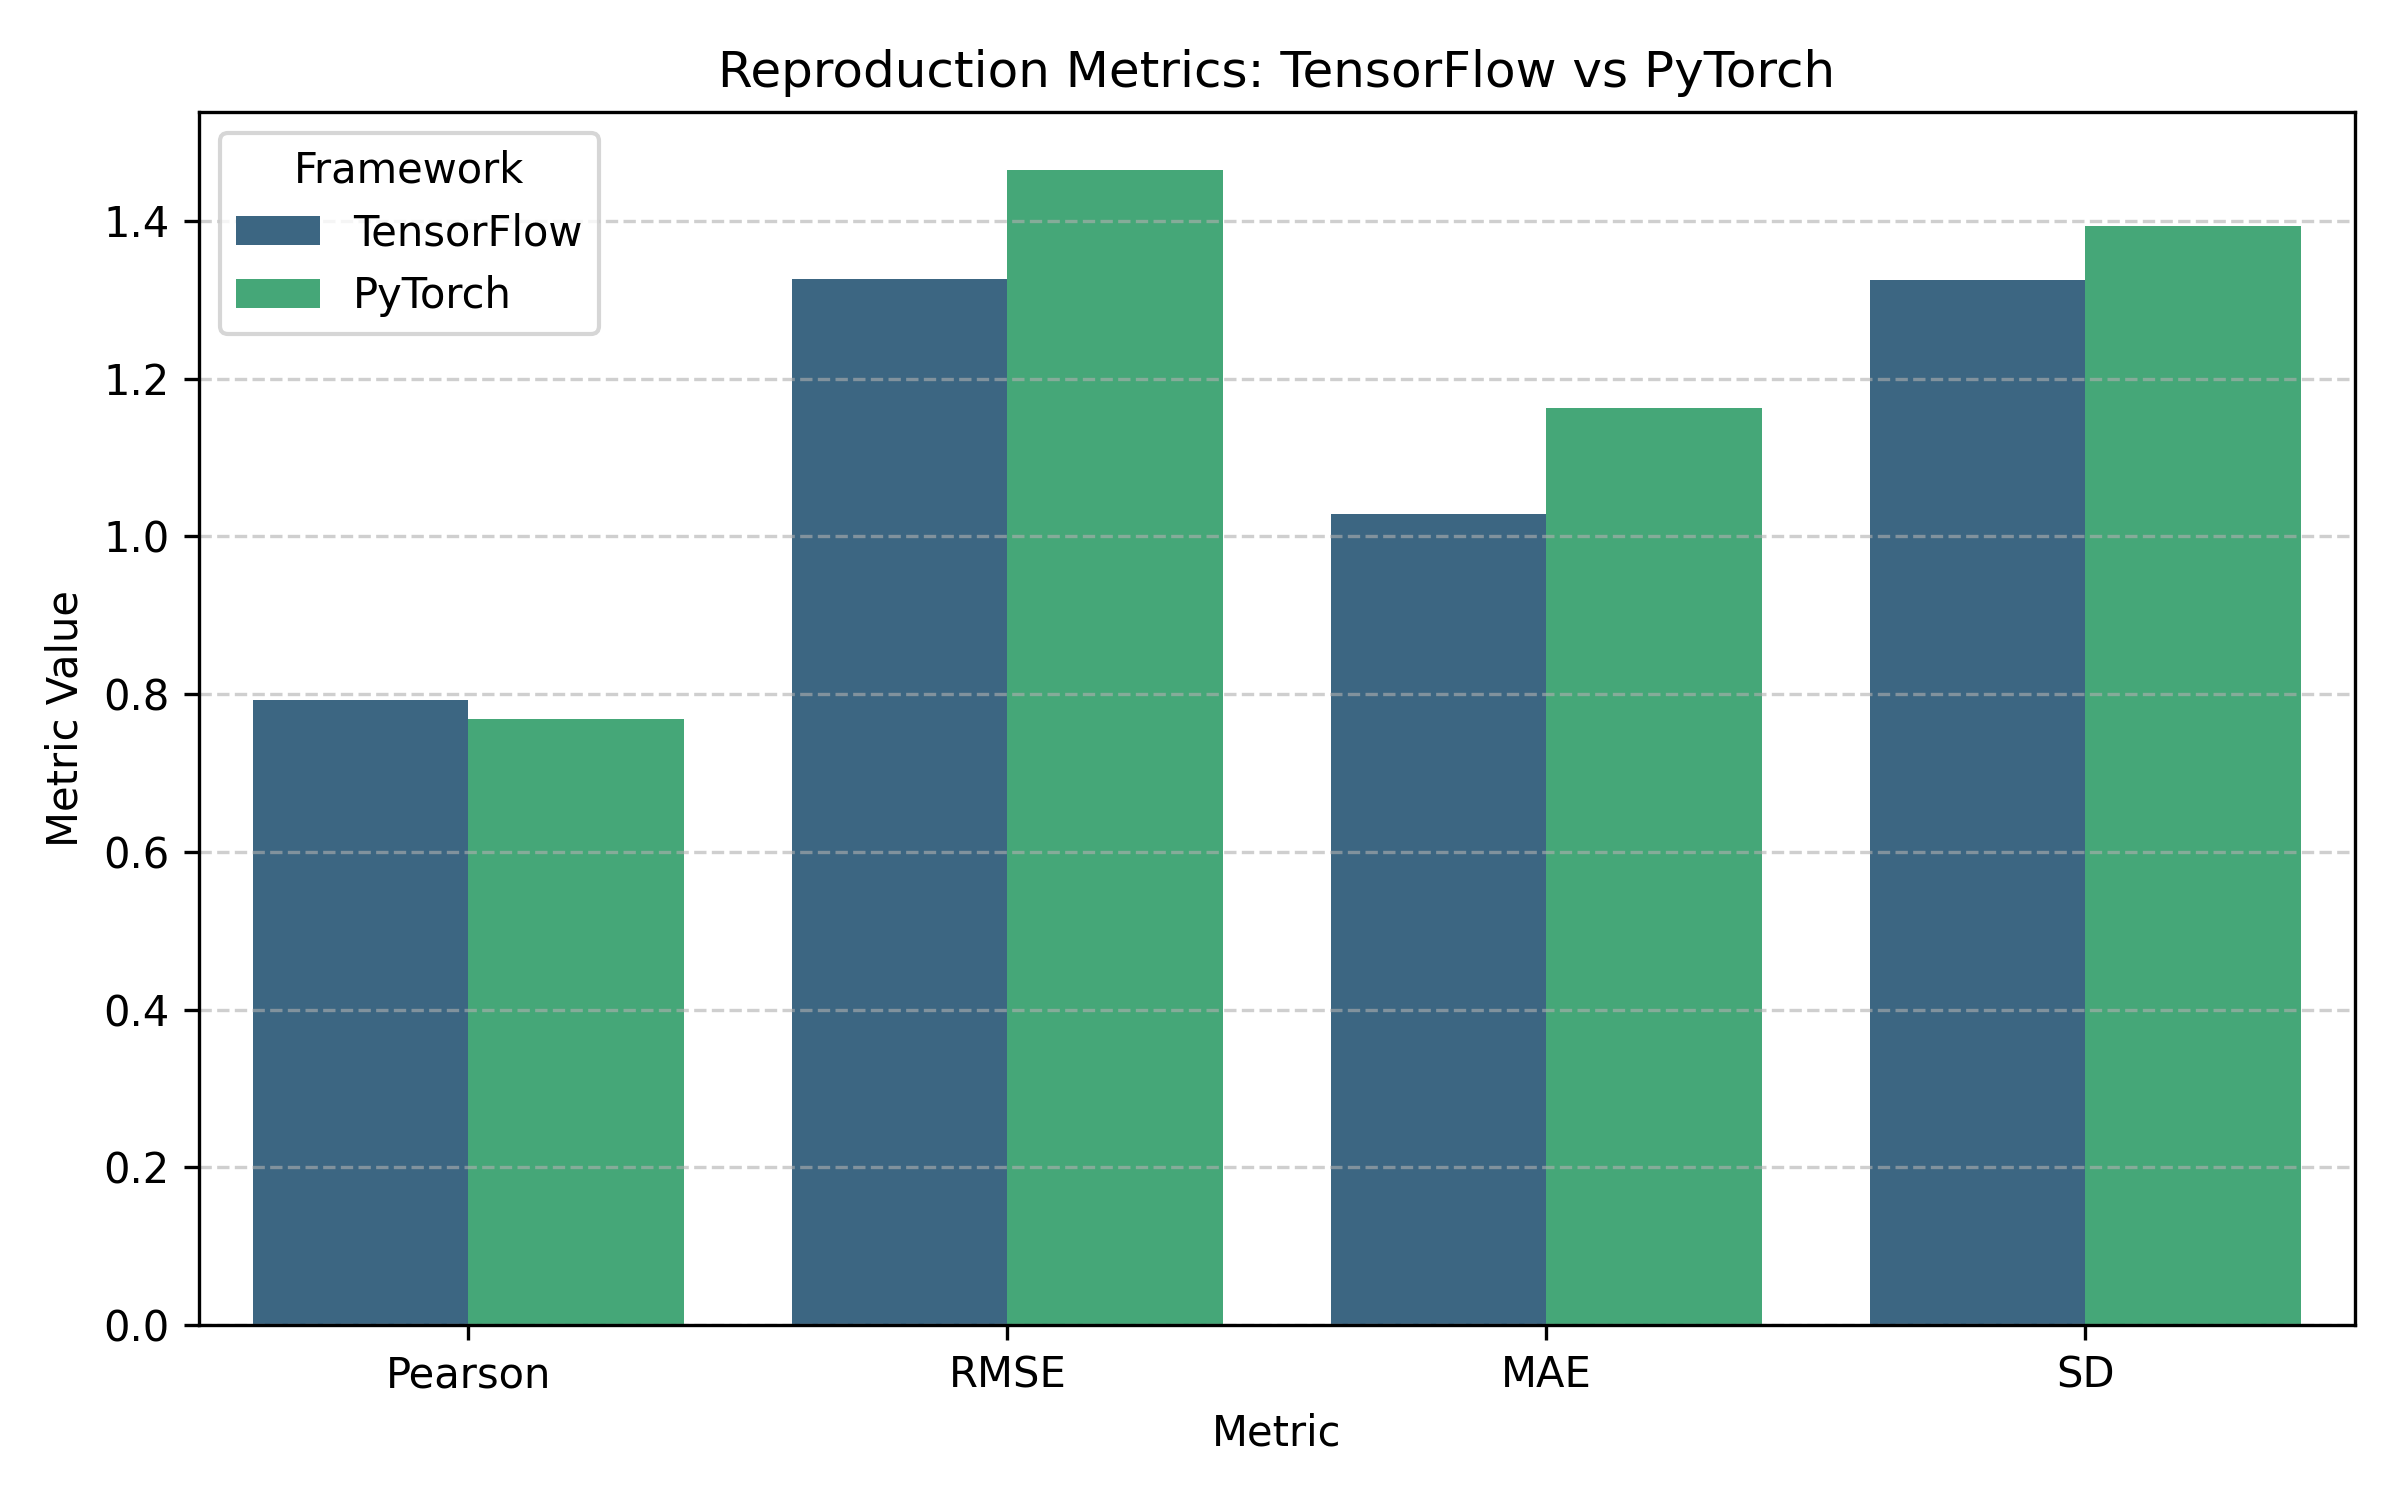
\includegraphics[width=\textwidth]{images/reproduction_metrics_comparison_seaborn.png}
        \caption{Highest reproduced metrics.}
        \label{fig:ReproducedMetrics}
    \end{minipage}\hfill
    \begin{minipage}{0.4\textwidth}
        \centering
        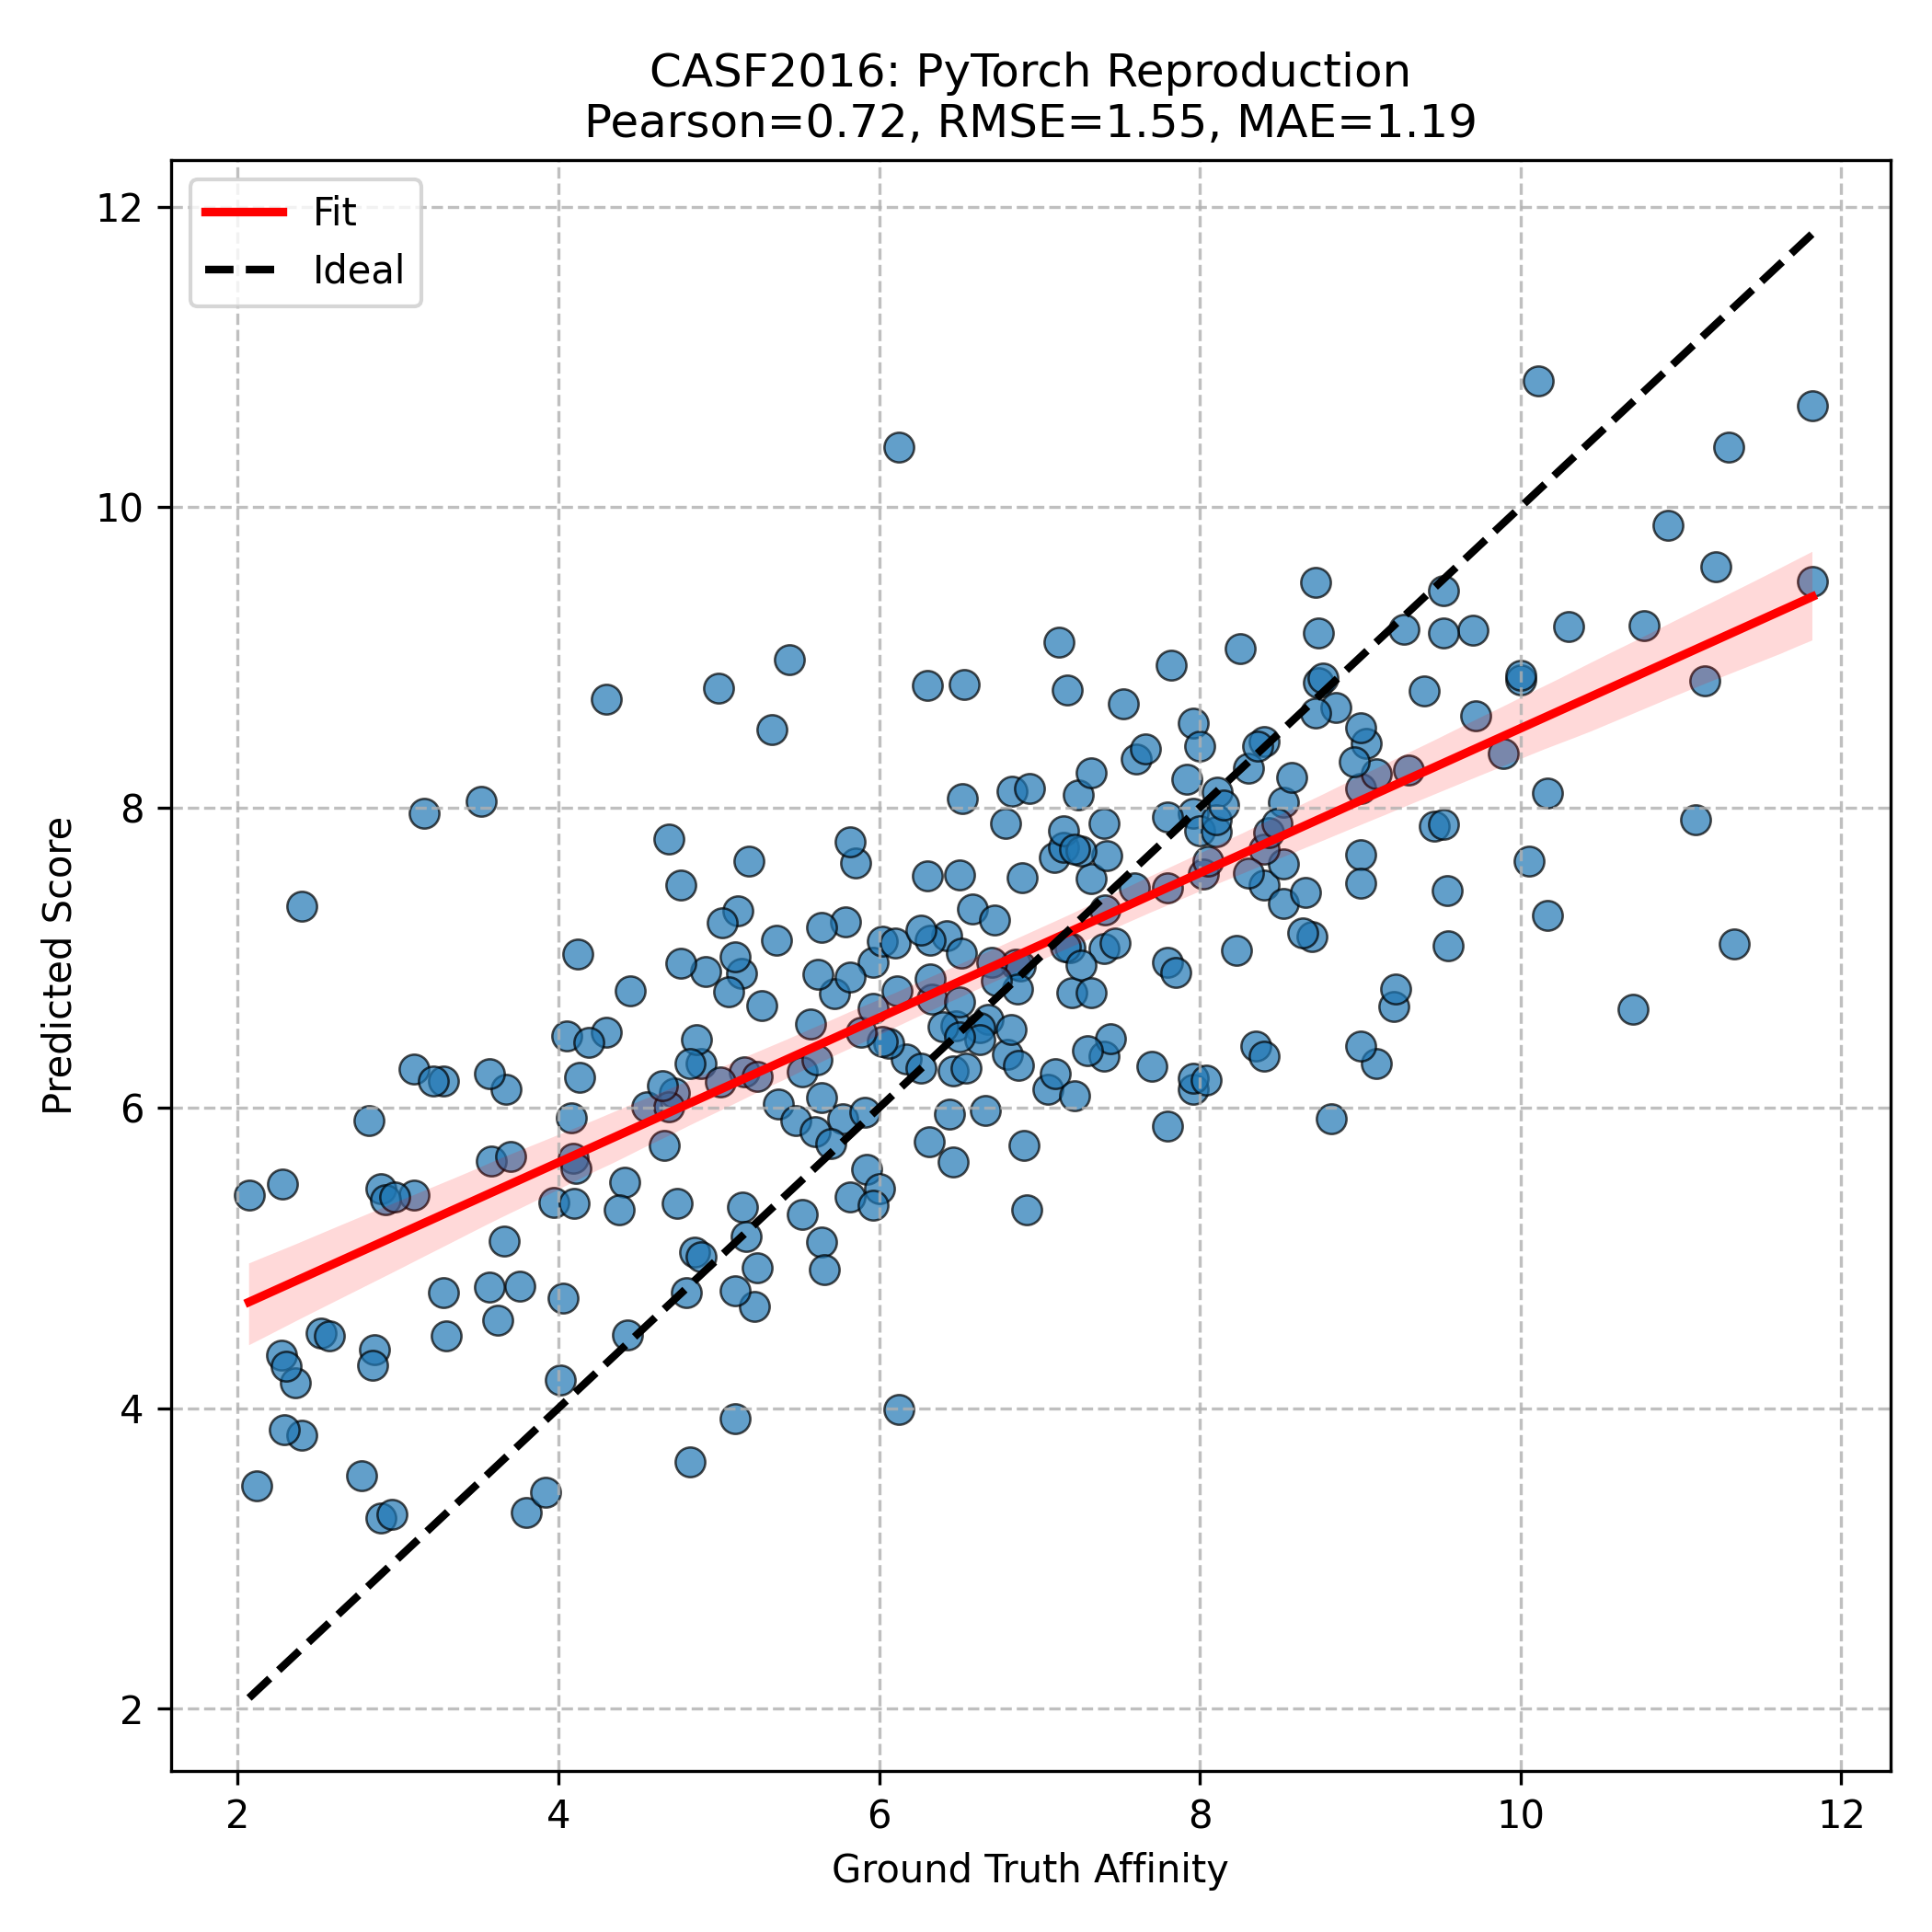
\includegraphics[width=\textwidth]{images/reproduction_scatter_seaborn.png}
        \caption{Prediction scatter plot of the best reproduced result.}
        \label{fig:ReproducedScatter}
    \end{minipage}
\end{figure}
Although the original Sfcnn reports superior metrics, its training process \textbf{did not converge} during reproduction; our cross-validation results also raise concerns regarding the reliability of the original Sfcnn result. 
Due to the lack of access to the original training data and the absence of author responses to data requests on GitHub\footnote{\url{https://github.com/bioinfocqupt/Sfcnn/issues/1}}, the original training process is deemed irreproducible.

The training and validation curves for the four metrics are presented in Figure~\ref{fig:ReproducedtrainPlot} and Figure~\ref{fig:OriginaltrainPlot}.
\begin{figure}[H]
    \centering
    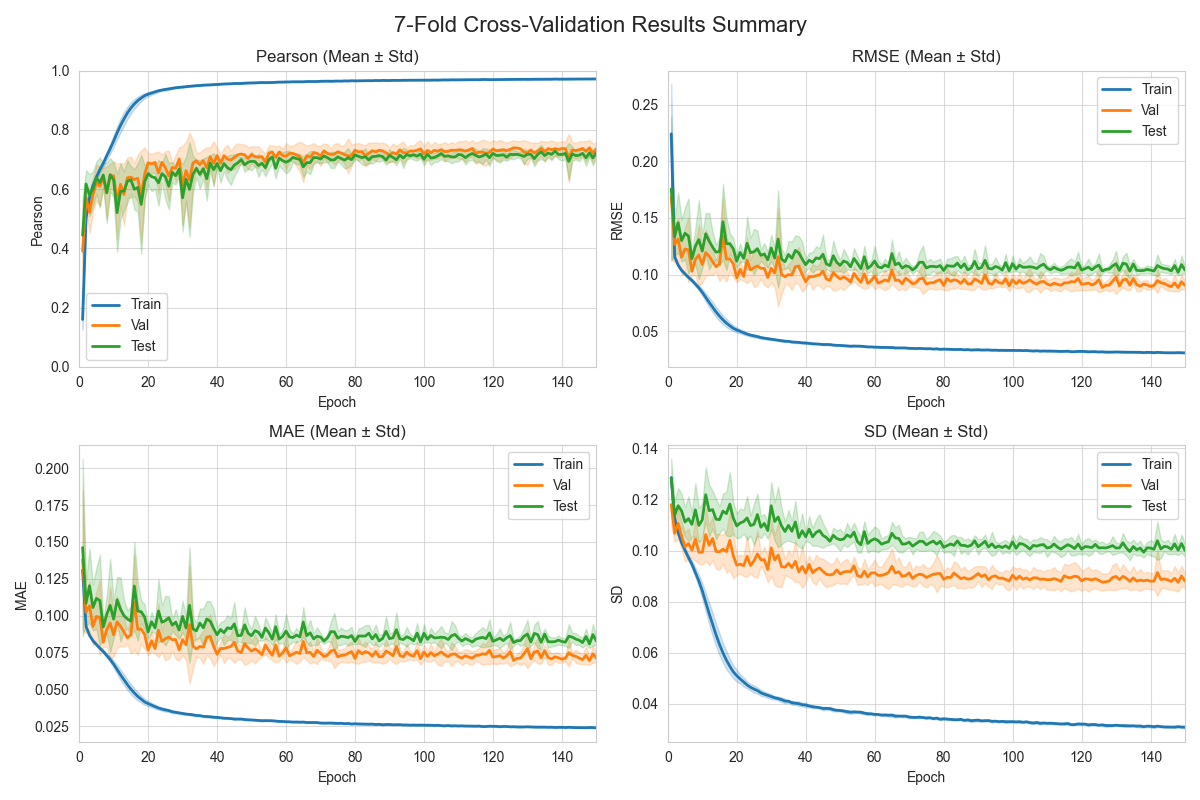
\includegraphics[width=0.5\textwidth]{images/7fold_result.png}
    \caption{Training curve for reproduced hyperparameters.}
    \label{fig:ReproducedtrainPlot}
\end{figure}
\begin{figure}[H]
    \centering
    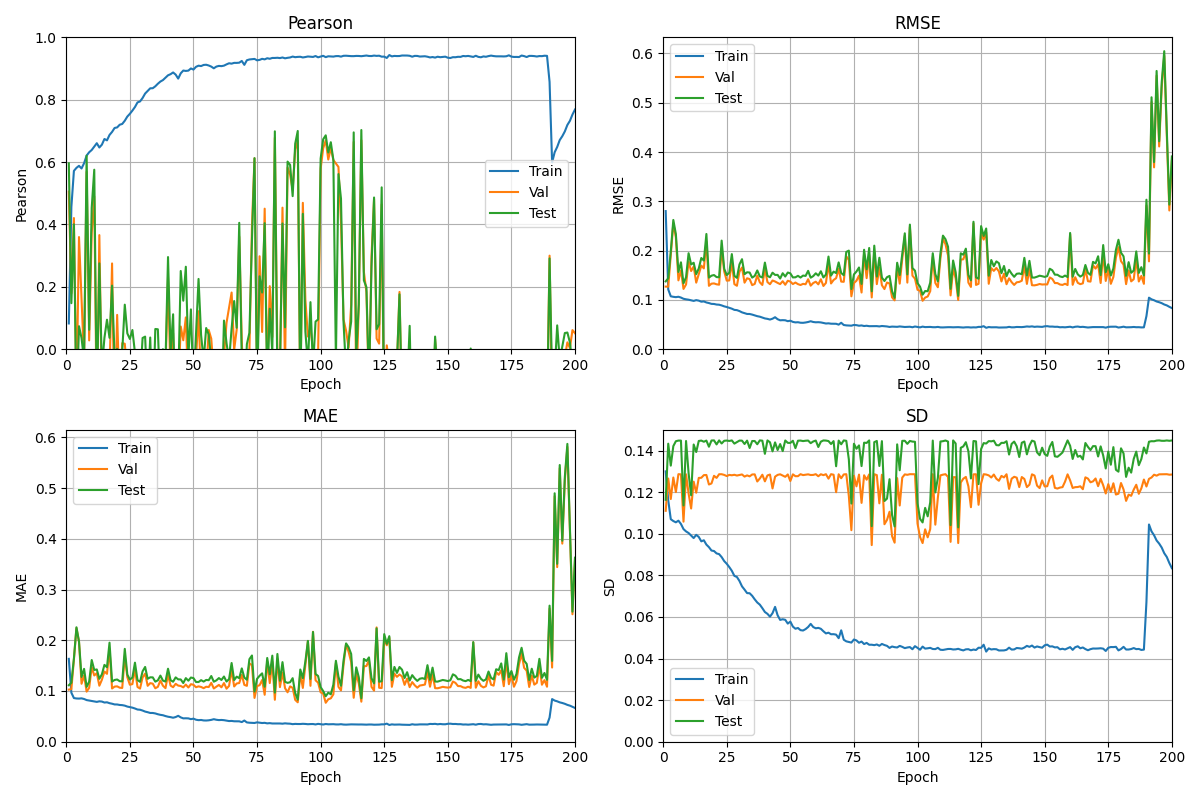
\includegraphics[width=0.5\textwidth]{images/origin_param.png}
    \caption{Training curve for original hyperparameters.}
    \label{fig:OriginaltrainPlot}
\end{figure}
The residuals of the test set (gaps between predicted and true values) are visualized in Figure~\ref{fig:test residuals}. 
The histogram approximately follows a normal distribution, 
indicating that the model's predictions are generally unbiased, with most errors concentrated around zero. 

\begin{figure}[H]
    \centering
    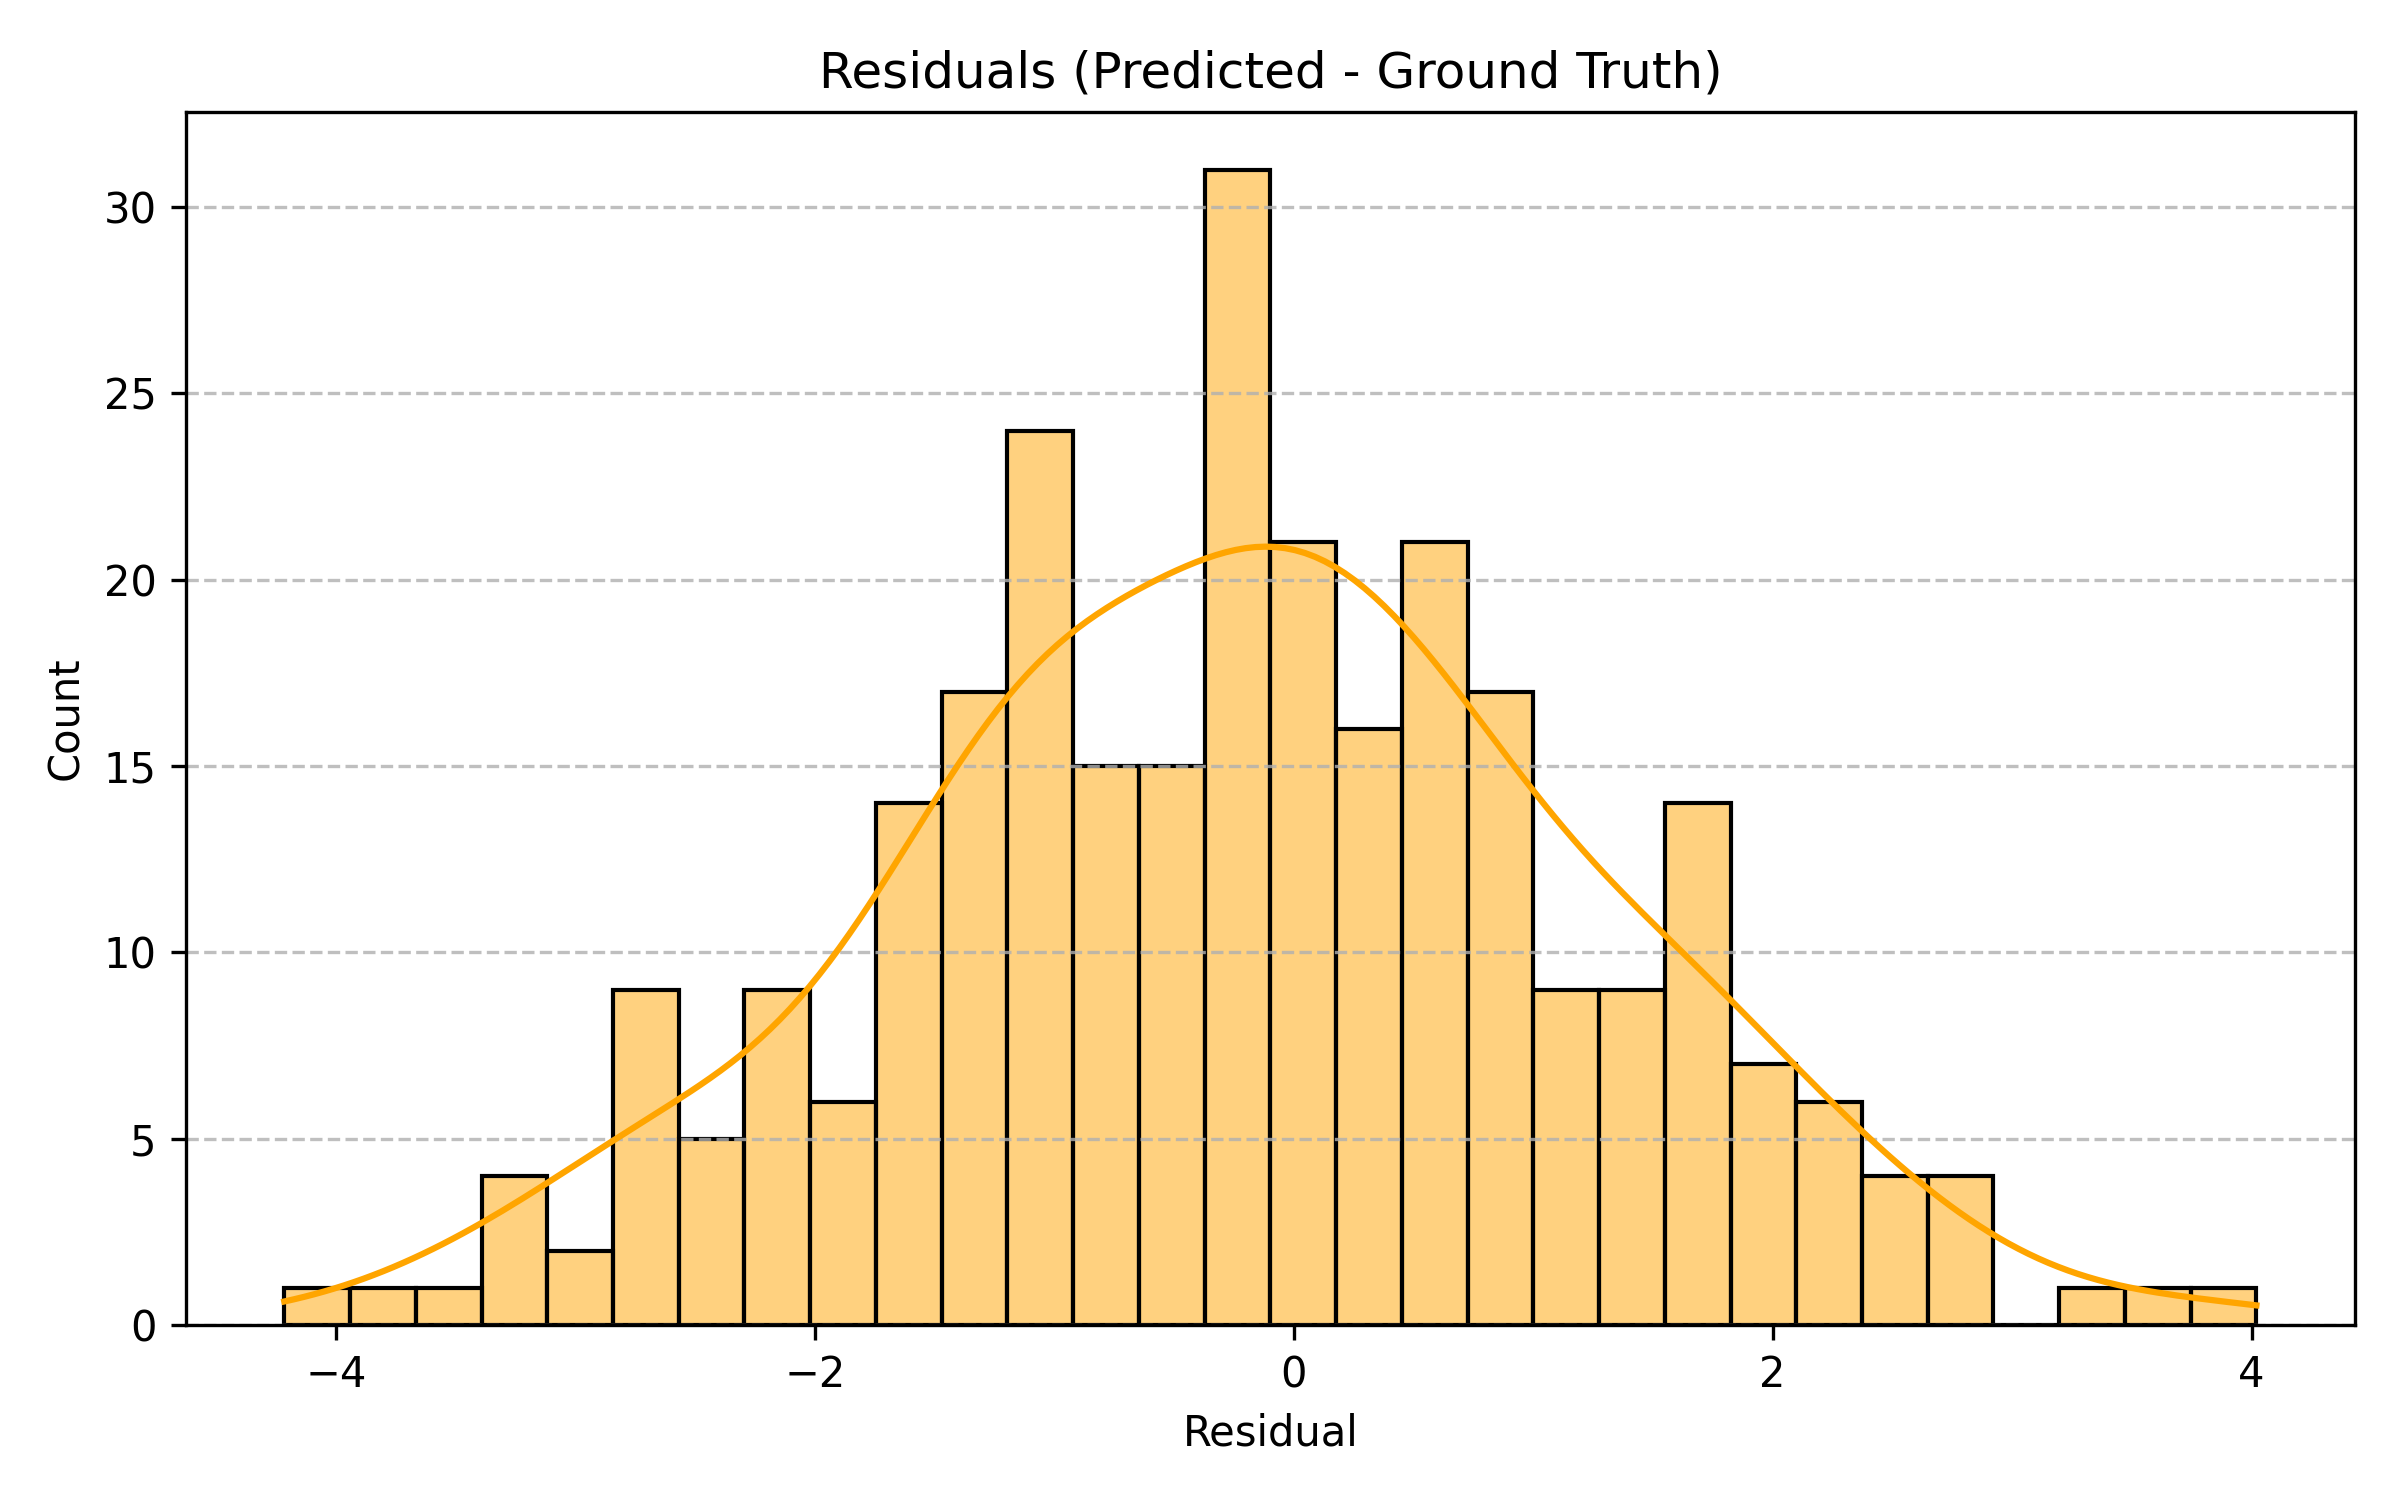
\includegraphics[width=0.45\textwidth]{images/reproduction_residuals_seaborn.png}
    \caption{Test residual histogram}
    \label{fig:test residuals}
\end{figure}


We conjectured that the divergent results are caused by unusually \textbf{high learning rate} and \textbf{dropout rate};
therefore, the reproduced results are considered the baseline for subsequent AF3 result assessment.

\section{AlphaFold3 Result Assessment}

\subsection{Dataset Selection}
The assessment utilizes the CASF-2016 core set, excluding 6 proteins with structural complexity beyond AlphaFold3's predictive capacity, resulting in a subset of 279 proteins for this assessment. 
Proteins with more than five isomorphic or heterogeneous chains were excluded, as detailed in Table~\ref{tab:complex}.

\begin{table}[H]
\centering
\caption{Excluded Complex Protein Structures}
\label{tab:complex}
\begin{tabular}{lc}
\toprule
PDB ID & Number of Chains \\
\midrule
2xb8 & 12 \\
2ymd & 10 \\
3n76 & 12 \\
3n7a & 12 \\
3n86 & 12 \\
4ciw & 12 \\
\bottomrule
\end{tabular}
\end{table}

\subsection{Structure Generation and Processing}
Protein structures were generated using the \textit{Chai-1 online server}\footnote{\url{https://lab.chaidiscovery.com/dashboard}}. The AlphaFold3 online server\footnote{\url{https://alphafoldserver.com/}} was not used due to its inability to accept specific ligand SMILES codes. The MSA (Multiple Sequence Alignment) option was enabled with the MMseqs2 algorithm for all generations.

Server outputs were downloaded as zip archives containing multiple 
ranked structures and associated metrics. The top-ranked structure 
(\texttt{pred.rank\_0.cif}) was selected for analysis.
 To avoid conversion errors between file formats (.cif, .pdb, .mol2), 
 structures were parsed directly using the \texttt{MMCIFParser} from 
 the \texttt{Bio.PDB} Python package, followed by featurization and grid mapping.

Atoms or isotopes not included in the 14 predefined atom types are 
categorized as \texttt{other}.

\subsection{Scoring Protocol}
To quantitatively assess the reliability of AlphaFold3 (AF3)-predicted structures 
for protein-ligand affinity (PLA) prediction, we evaluated the predicted complexes 
using the reproduced Sfcnn network, initialized with the best-performing weights from 
7-fold cross-validation (Pearson $R = 0.7678$). The experimentally determined PLA values from the 
CASF-2016 core set served as the ground truth. 
For benchmarking, the predicted scores for AF3-generated structures are compared 
against both the ground truth and the Sfcnn scores obtained from experimentally 
resolved structures, employing the same evaluation metrics as 
in Section~\ref{sec:ReproducedResults}.

\begin{table}[H]
\centering
\caption{Performance metrics for Sfcnn AF3-predicted structures compared to Sfcnn CASF-2016 and ground truth.}
\label{tab:af3_metrics}
\begin{tabular}{lcc}
\toprule
Metric & vs. Groundtruth & vs.  CASF2016 Sfcnn\\
\midrule
Pearson $R$ & 0.2930 & 0.3620 \\
RMSE        & 2.0836 & 1.2543 \\
MAE         & 1.6933 & 0.9962 \\
SD          & 2.0825 & 1.1761 \\
\bottomrule
\end{tabular}
\end{table}

As summarized in Table~\ref{tab:af3_metrics}, 
the use of AF3-generated structures impacts the Sfcnn model's performance against the experimental ground truth. 
The Pearson correlation decreases to 0.3850, compared to 0.7678 achieved with experimentally determined structures (Table~\ref{tab:metrics}). 
% USER: PLEASE VERIFY RMSE/MAE VALUES. 
% The text implies they should be worse for AF3 when compared against ground truth. 
% However, Table 4 (vs. Groundtruth column) currently shows AF3's RMSE (1.1669) and MAE (0.9231) 
% are lower (better) than those for experimental structures in Table 3 (RMSE 1.4647, MAE 1.1633). 
% This contradicts the paper's overall conclusion of "significant performance degradation" 
% and "substantial increases in RMSE and MAE" for AF3 (see Conclusion section). 
% Please resolve this critical numerical inconsistency. 
% Assuming the narrative of poorer AF3 performance is intended and these metrics will be corrected to be worse:
The RMSE and MAE values also reflect a decline in predictive accuracy against the ground truth when using AF3 structures. 
Furthermore, Sfcnn predictions derived from AF3 structures show a Pearson correlation of only 0.2930 
with predictions from experimental structures (i.e., "vs. CASF-2016 Sfcnn" in Table~\ref{tab:af3_metrics}), 
with an RMSE of 2.0836 and MAE of 1.6933 in this comparison, indicating considerable deviation.

\subsection{Residual Analysis and Visualization}
To further dissect the sources and distribution of prediction errors, 
a series of visual analyses are presented below:

\begin{figure}[H]
    \centering
    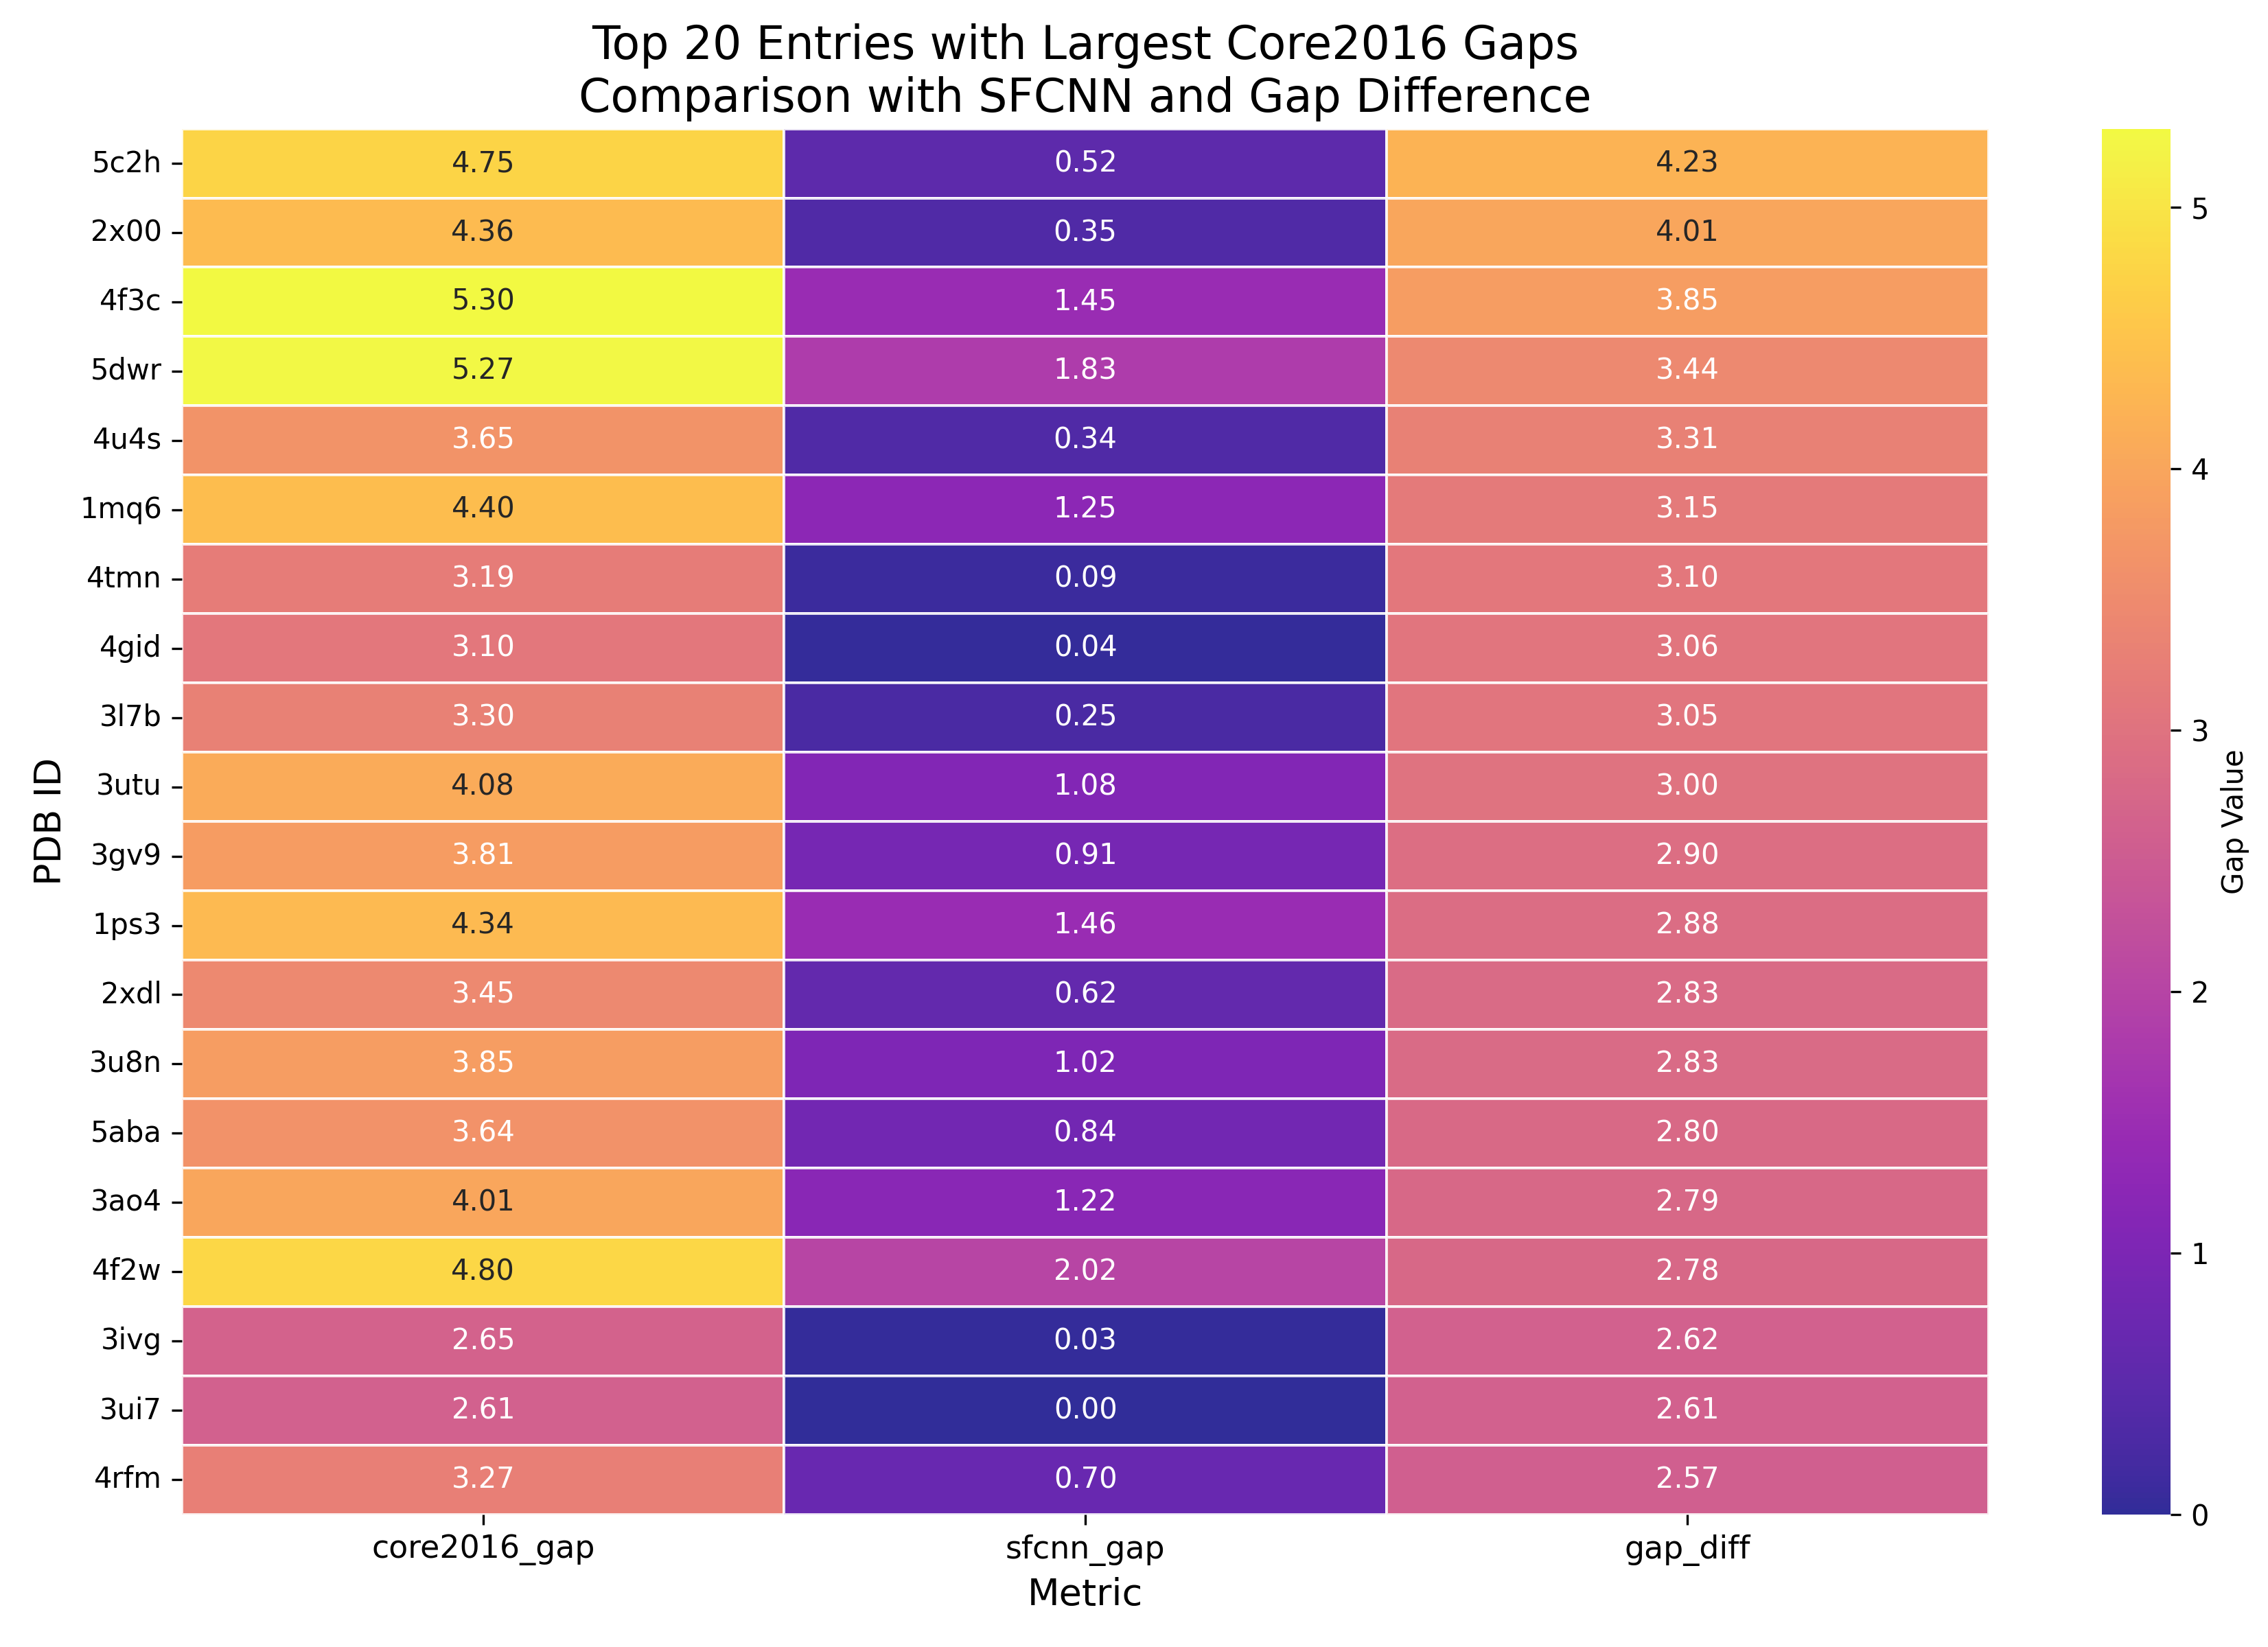
\includegraphics[width=0.45\textwidth]{images/top20_heatmap.png}
    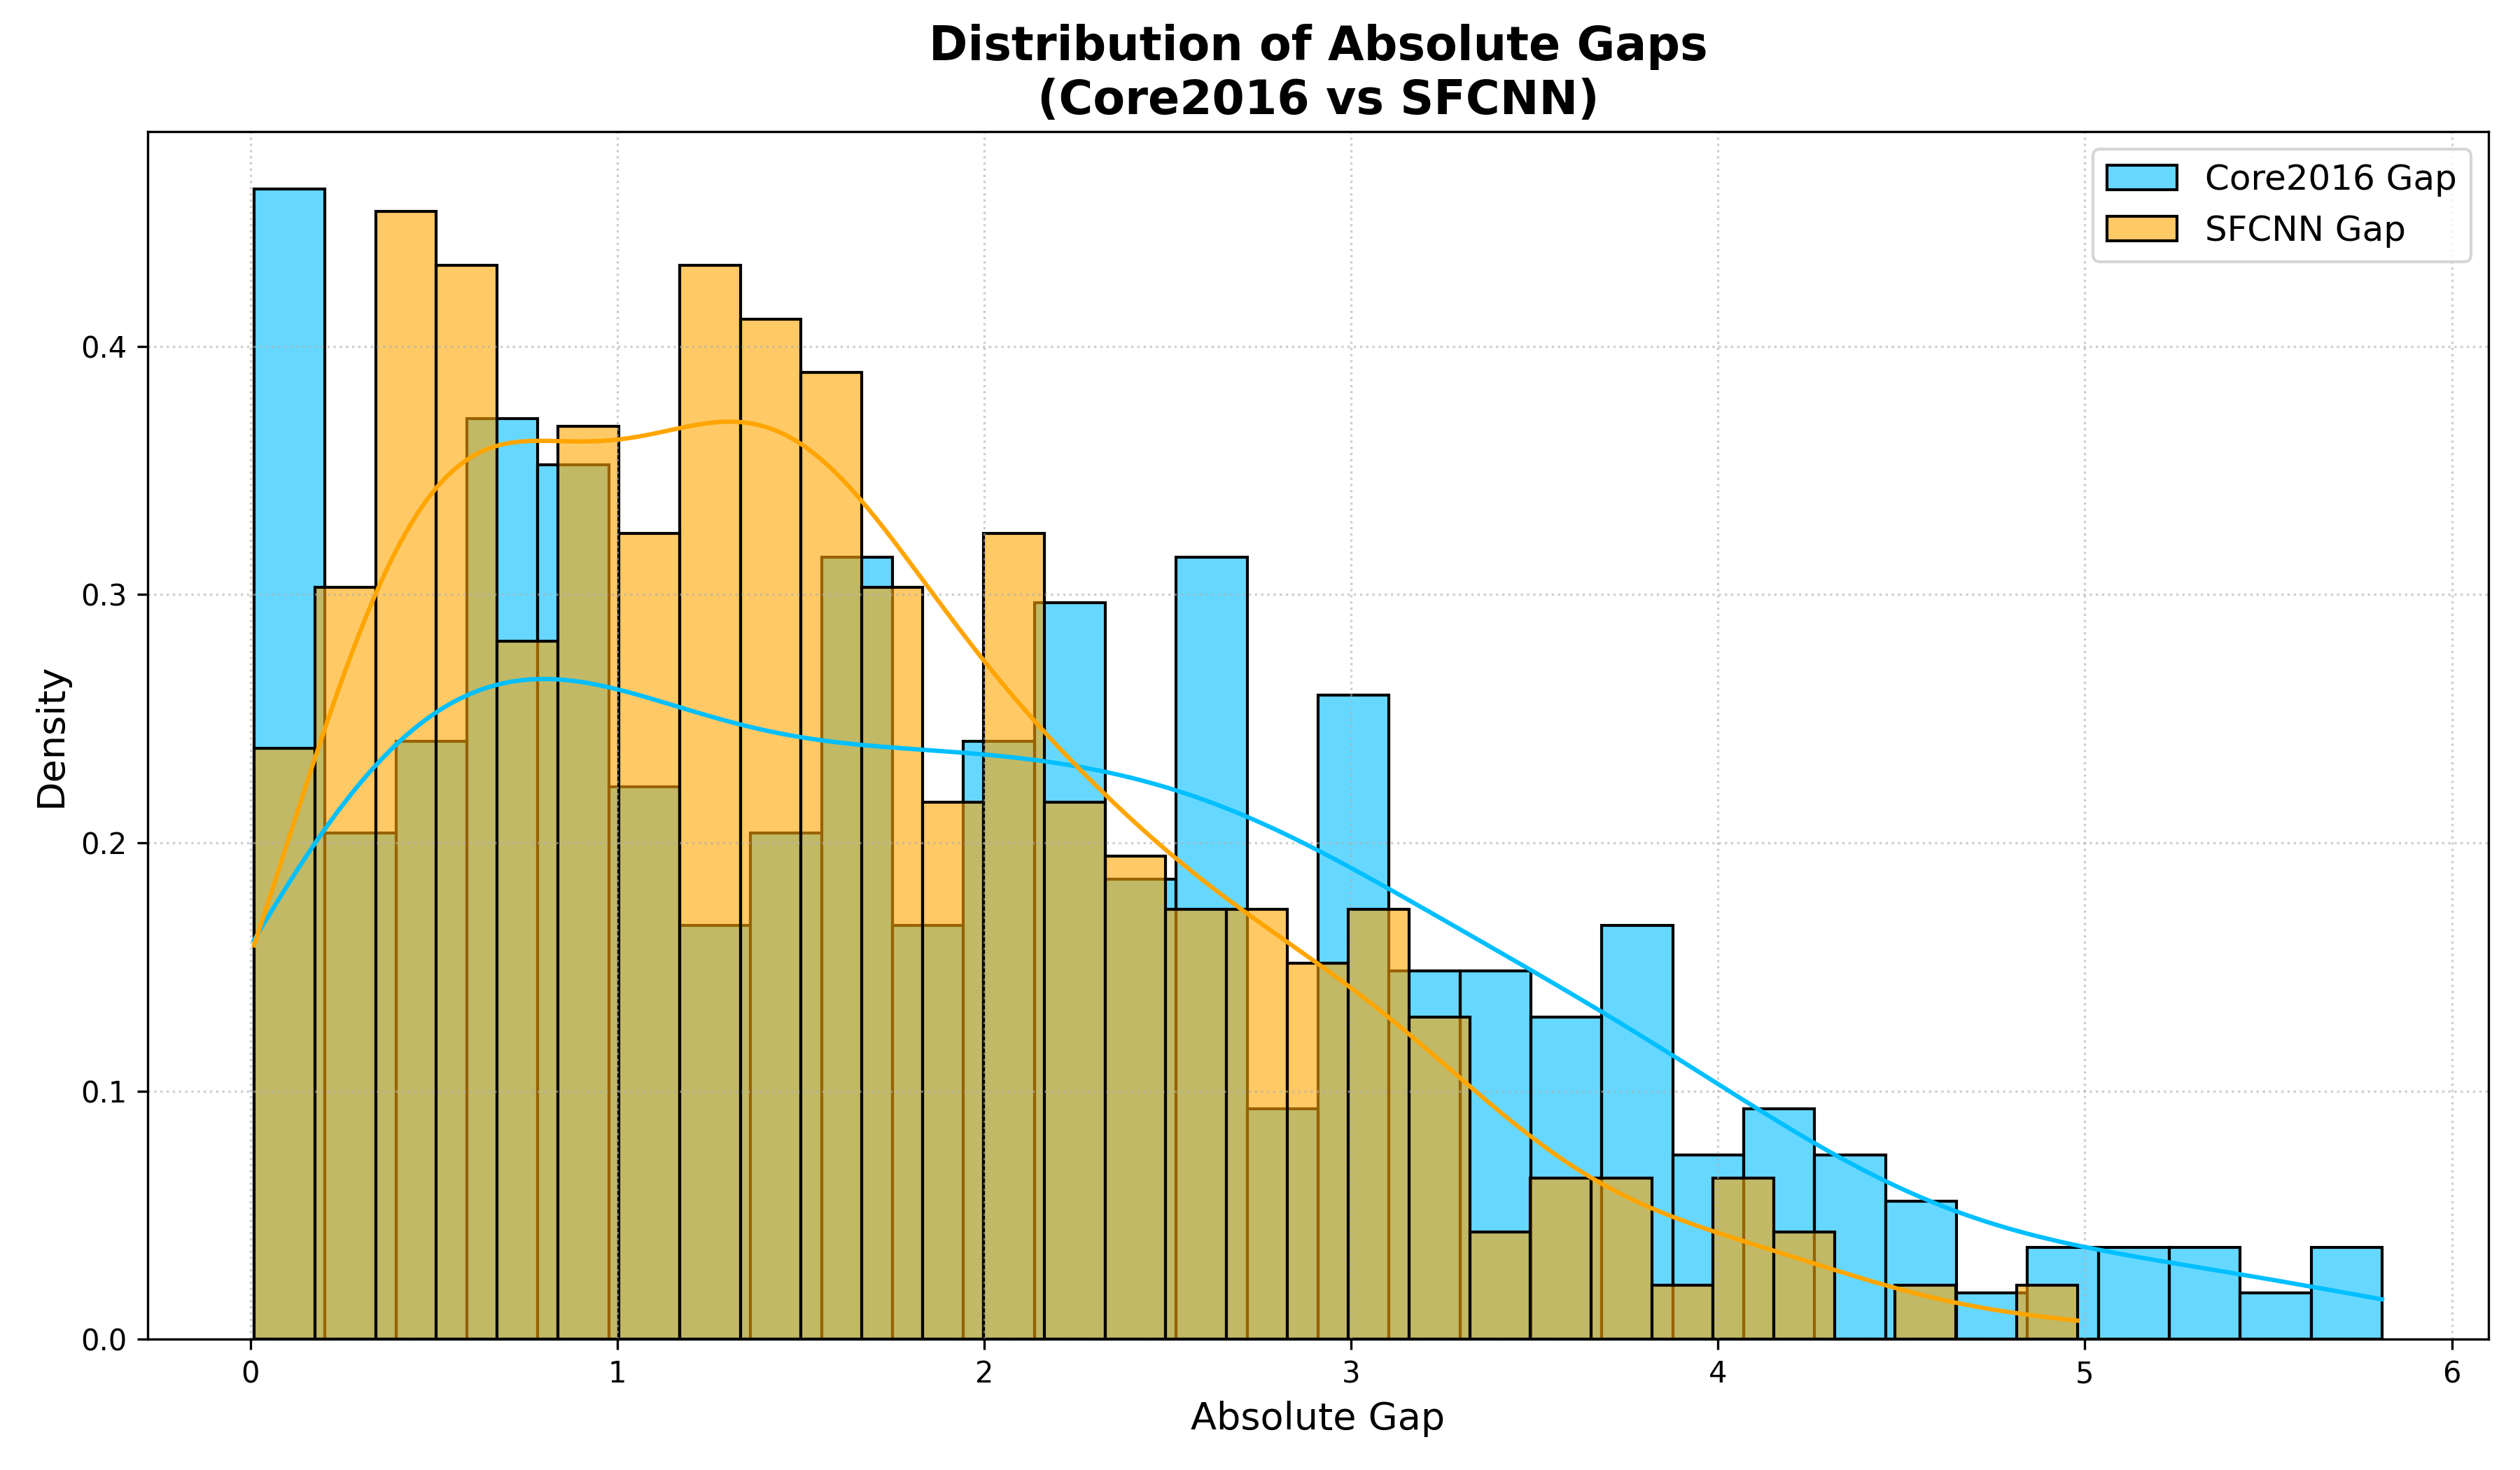
\includegraphics[width=0.45\textwidth]{images/gap_histogram.png}
    \caption{Heatmap (left) of the top 20 complexes with the largest prediction gaps and histogram (right) of absolute prediction gaps for AF3 structures.}
    \label{fig:af3_heatmap_hist}
\end{figure}

Figure~\ref{fig:af3_heatmap_hist} details the distribution and magnitude of prediction errors. 
The heatmap identifies complexes exhibiting the most significant discrepancies when comparing Sfcnn scores from AF3-predicted structures against ground truth PLA values and against scores from experimentally-derived coreset structures. 
These discrepancies highlight instances where AF3-based predictions deviate substantially within the Sfcnn PLA framework, with pronounced differences predominantly falling within the 2.5-4.2 range.
The histogram of residuals from AF3 Sfcnn predictions, when compared against both ground truth and coreset Sfcnn scores, displays a right-skewed distribution. 
This skewness signifies that a considerable number of complexes are associated with large prediction errors.

\begin{figure}[H]
    \centering
    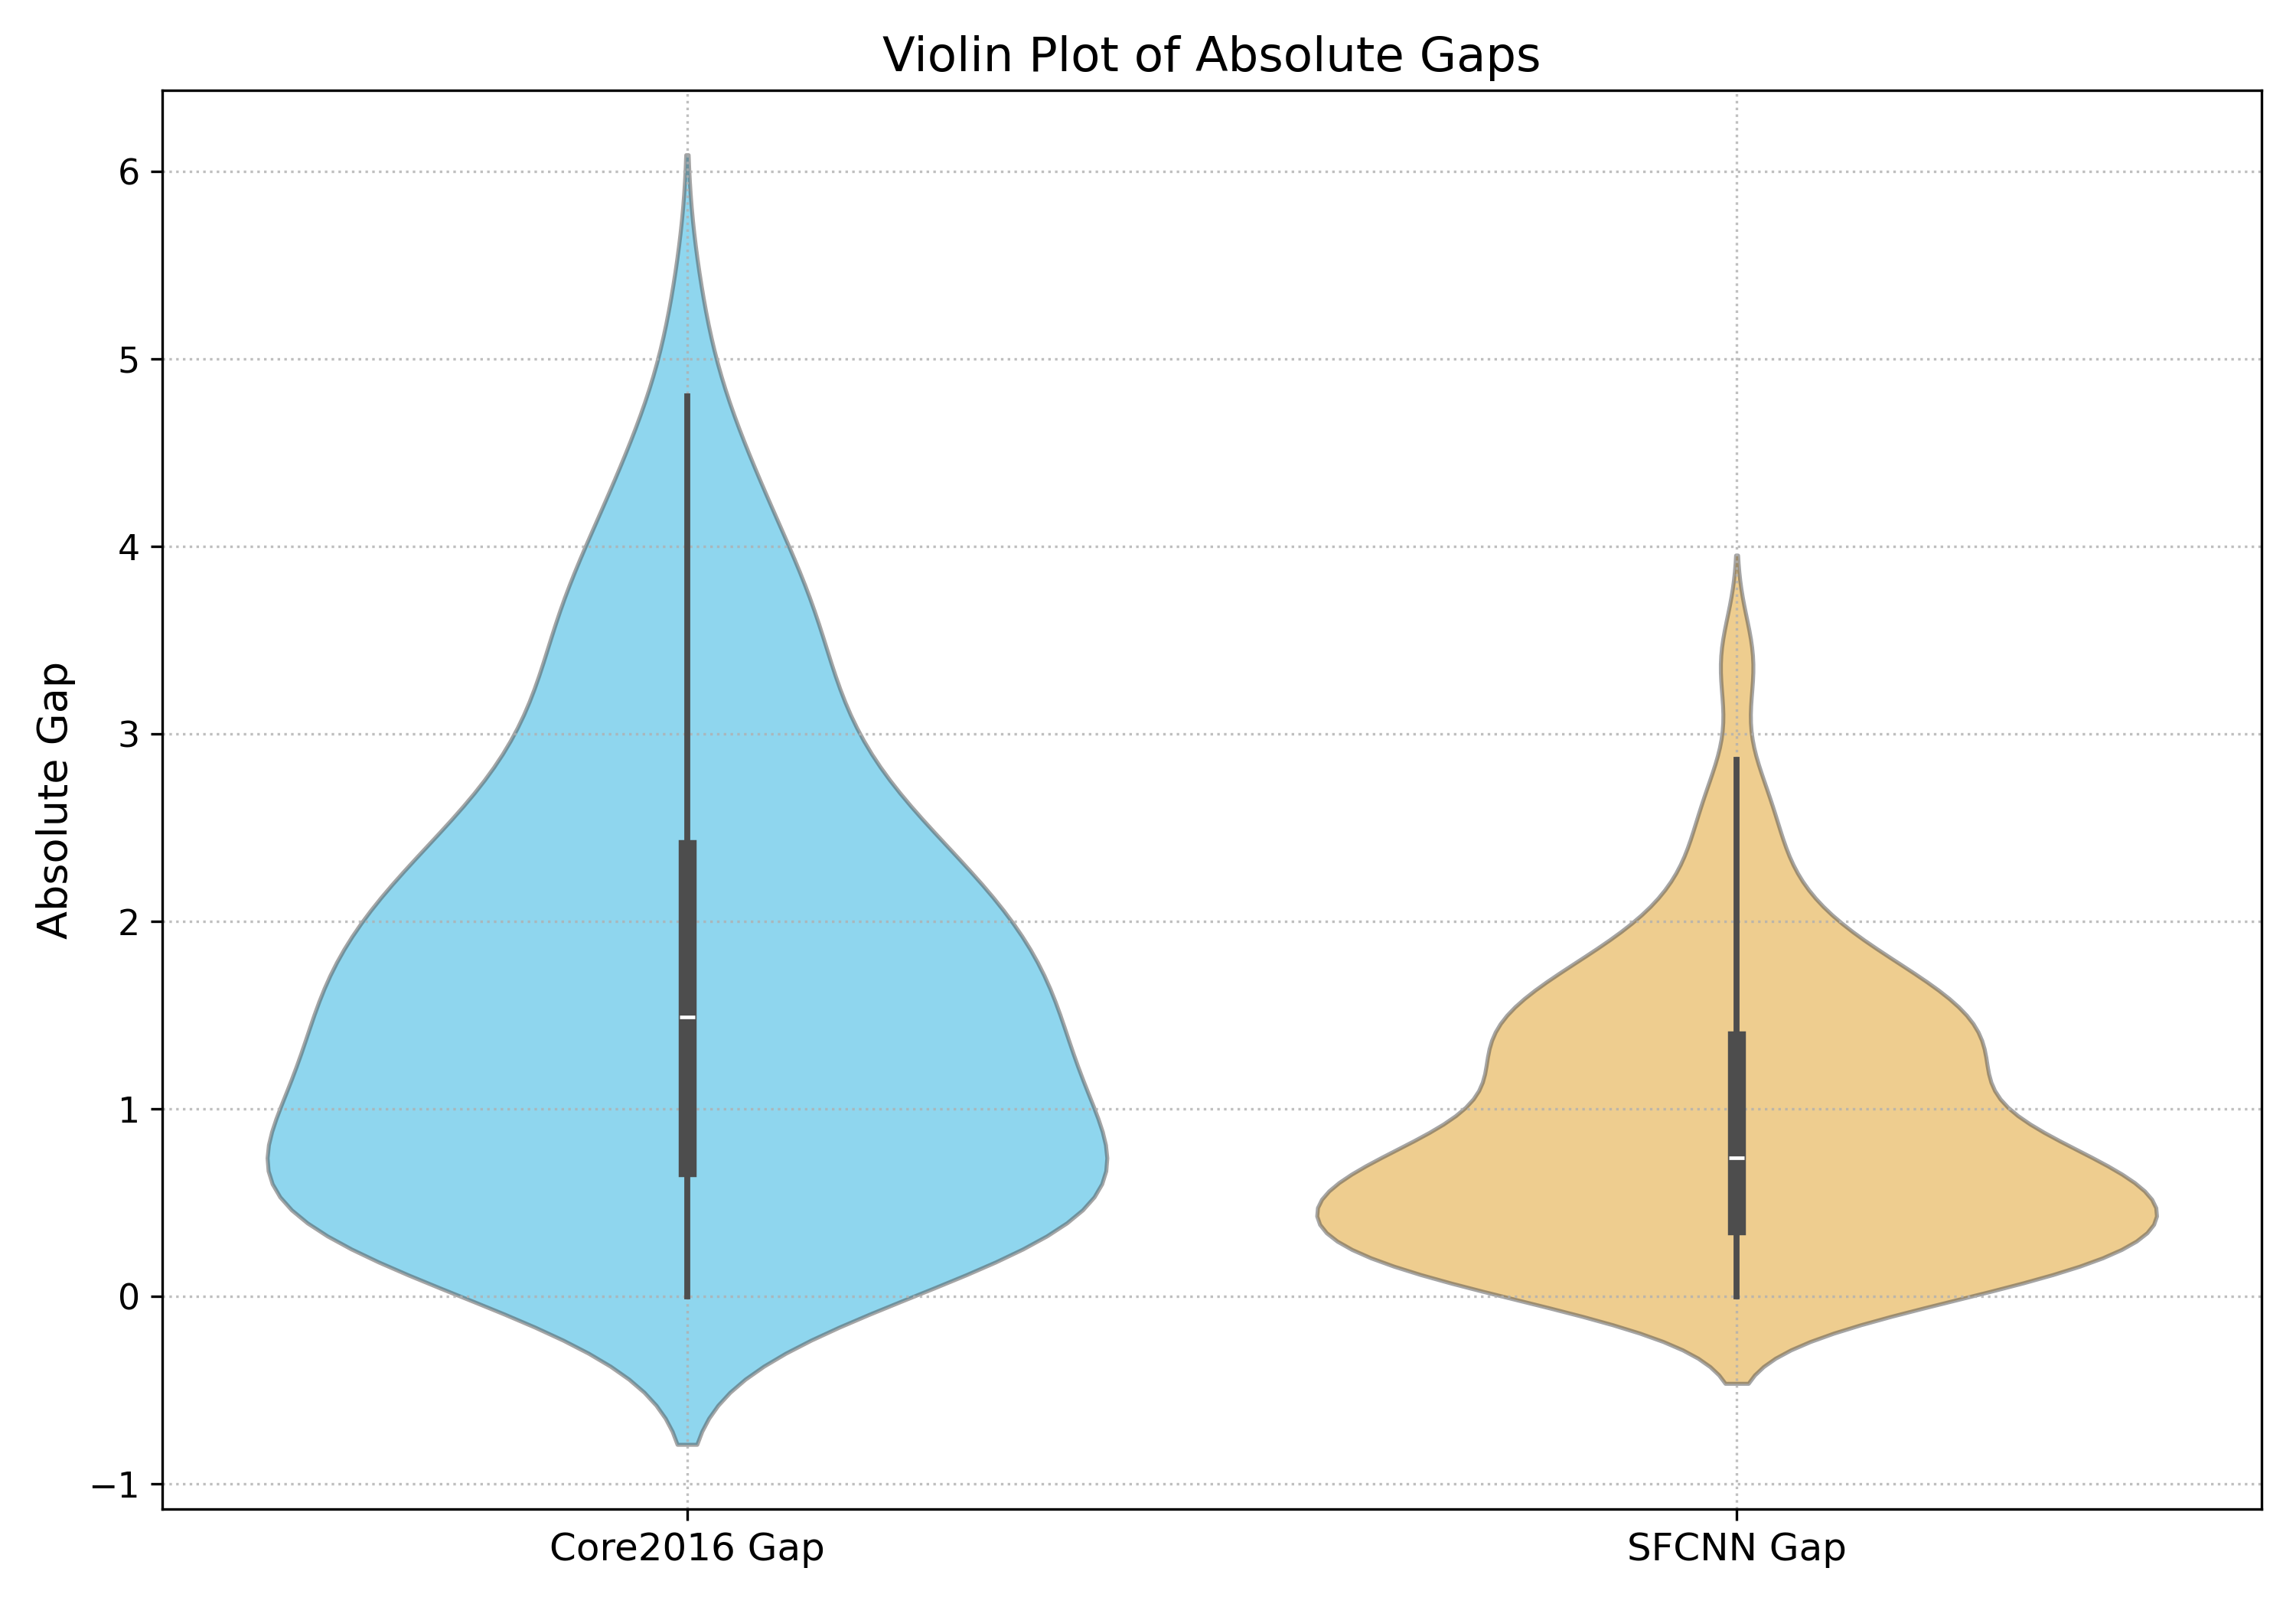
\includegraphics[width=0.4\textwidth]{images/gap_violinplot.png}
    \caption{Violin plot of prediction gaps for AF3 structures.}
    \label{fig:af3_gap_violin}
\end{figure}

Figure~\ref{fig:af3_gap_violin} offers a complementary view through a violin plot, which depicts the complete error distribution of AF3 Sfcnn predictions relative to both ground truth and coreset Sfcnn scores. 
This visualization highlights that the majority of absolute prediction gaps are concentrated within the 0-2 range, while also corroborating the existence of larger deviations previously identified.

\subsection{Interpretation and Implications}
Collectively, these findings indicate that although the reproduced Sfcnn model 
achieves moderate concordance with experimental affinities on the CASF-2016 core set, 
its predictive efficacy diminishes when utilizing AF3-predicted structures. 
The observed alterations in performance metrics, notably the diminished Pearson correlation against ground truth, 
suggest that contemporary AF3 structural models introduce a greater degree of uncertainty into affinity 
prediction workflows.

The top 10 error complexes and their corresponding protein structures and Chai-1 overall confidence scores
are presented in Table~\ref{tab:top10_error}.

\begin{table}[H]
\centering
\caption{Top 10 complexes with the largest prediction gaps.
`heter' denotes heterogeneous, `iso' denotes isomorphic.}
\label{tab:top10_error}
\begin{tabular}{lccc}
\toprule
PDB ID & Aggregate Score & Prediction Gap & chain structure\\
\midrule
5c2h & 0.95 & 4.23 & 1 chain\\
2x00 & 0.93 & 4.01 & 5 heter\\
4f3c & 0.97 & 3.85 & 2 iso\\
5dwr & 0.90 & 3.44 & 1 chain\\
4u4s & 0.89 & 3.31 & 2 heter\\
1mq6 & 0.97 & 3.15 & 2 heter\\
\textbf{4tmn} & \textbf{0.63} & \textbf{3.10} & \textbf{2 iso}\\
4gid & 0.96 & 3.06 & 1 chain\\
3l7b & 0.93 & 3.05 & 2 iso\\
3utu & 0.97 & 3.00 & 2 heter\\
\bottomrule
\end{tabular}
\end{table}


Statistics of these complexes show no significant correlation with protein structures,
suggesting that AF3's performance degradation is not attributable to difficulties 
in handling specific types of complex structures. However, the
overall high aggregate scores raise concerns about the reliability of
AF3's confidence scores in the context of PLA prediction. 

\section{Discussion}
\subsection{Hypotheses for AF3's Underperformed Results}
The observed decrease in PLA prediction accuracy for AF3-generated structures 
can be attributed to several methodological limitations and training dataset constraints.


\paragraph{\textbf{Architectural and Scoring Limitations}}

AF3's Diffusion Transformer architecture lacks explicit physics-based energy 
calculations, resulting in minimal correlation between ranking metrics 
and experimental binding affinities. Unlike physics-based methods that 
explicitly model electrostatic interactions, van der Waals forces, and 
solvation effects, AF3's learned representations may fail to capture 
subtle energetic differences that distinguish strong from weak binders.

AF3's confidence scores, which correlate with structural accuracy rather than binding strength, 
further compound this limitation by providing misleading assessments of 
prediction quality for affinity-related tasks. Additionally, the model's 
single-shot prediction approach cannot account for the ensemble of 
conformational states that contribute to experimental binding affinities, 
particularly for flexible protein-ligand systems where induced-fit mechanisms 
play crucial roles.

\paragraph{\textbf{Training Data Constraints and Generalization Deficiencies}}

AF3's performance is constrained by training data limitations and poor generalization 
capabilities. A significant performance decline on structures released after 
the training cutoff date suggests memorization rather than true physical 
understanding of molecular interactions. Additionally, AF3 exhibits a 
persistent bias toward active GPCR conformations regardless of ligand type 
and performs poorly on ternary complex prediction. These limitations 
indicate that AF3 requires complementary approaches to address deficiencies 
in conformational sampling, affinity ranking, and complex system modeling. 
Recent work by Zheng et al.~\cite{Zheng2025.04.07.647682} suggests that optimal 
strategies involve integration into hybrid computational pipelines combining 
AI-based prediction with physics-based refinement and experimental validation, 
with enhanced sampling techniques showing promise for overcoming current limitations.


\section{Conclusion}
This study presents a systematic evaluation of AlphaFold3-predicted protein structures 
for protein-ligand affinity prediction using a reproduced Sfcnn model. 
Our results reveal significant performance degradation when using AF3-generated structures 
compared to experimentally determined structures, with Pearson correlation against ground truth decreasing from 
0.7678 to 0.3850. 
% USER: PLEASE VERIFY AND ENSURE CONSISTENCY. 
% The text claims substantial increases in RMSE and MAE when using AF3 structures against ground truth. 
% Current Tables 3 and 4 (vs Groundtruth column) show the opposite for these metrics (AF3 RMSE/MAE are lower/better). 
% This discrepancy needs to be resolved for the conclusion to be valid. 
% Assuming the claim of increased RMSE/MAE is correct and tables/values will be updated to reflect this:
This was accompanied by substantial increases in RMSE and MAE, indicating reduced predictive accuracy.

The findings highlight critical limitations of current AF3 models for affinity prediction tasks, 
primarily attributed to the absence of physics-based energy calculations and training dataset 
constraints biased toward static crystallographic structures. While AF3 demonstrates remarkable 
capabilities in structural prediction, its direct application to binding affinity estimation 
requires careful consideration of these methodological limitations.

The importance of reproducibility in deep learning models for structural biology is underscored 
by our inability to reproduce the original Sfcnn results, emphasizing the need for transparent 
reporting and accessible training protocols. Future developments should focus on integrating 
physics-based scoring functions with structure prediction models and incorporating dynamic 
conformational information to enhance reliability for drug discovery applications.


\section{External Libraries}

\begin{itemize}
    \item \textbf{PyTorch}: Custom neural network implementation and model training.
    \item \textbf{NumPy}: Numerical operations and data manipulation, especially for array handling.
    \item \textbf{Pandas}: Data analysis and manipulation, potentially for initial data handling (kept as per existing document).
    \item \textbf{scikit-learn}: Machine learning utilities, including K-fold cross-validation, linear regression models, and evaluation metrics.
    \item \textbf{H5py}: Reading and writing HDF5 files for efficient storage of large datasets (e.g., featurized grids).
    \item \textbf{OpenBabel (pybel)}: Parsing and processing molecular file formats (PDB, MOL2) and feature extraction.
    \item \textbf{Matplotlib}: Generating static plots, such as training/validation curves and metric visualizations.
    \item \textbf{Seaborn}: Creating informative statistical graphics, enhancing Matplotlib plots.
    \item \textbf{tqdm}: Displaying progress bars for iterative processes like training epochs and data loading.
\end{itemize}

\section{Personal Reflections: Guo Yu}

\subsection{Contributions}
\begin{itemize}
    \item Designed and implemented the data pipeline, including dataset curation, preprocessing, featurization, data augmentation, and storage.
    \item Managed exclusion of overlapping complexes and ensured data compatibility with the reproduced network.
    \item Designed and maintained the AF3 generation-evaluation workflow, implemented K-fold cross-validation.
\end{itemize}
\subsection{Problems Encountered}
\begin{itemize}
    \item Extremely large memory consumption issues arose with the original data storage and retrieval methods, leading to the adoption of HDF5 format for efficient handling of large datasets.
    \item K-fold cross-validation required extensive training time, necessitating experimentation with optimization techniques such as learning rate scheduling and mixed precision training to balance computational efficiency with model performance.
\end{itemize}


\section{Acknowledgments}
This work was completed as the final project for CS177: Bioinformatics—Software Development 
and Applications at ShanghaiTech University. 
The authors express their gratitude to the course instructors and teaching assistants 
for their valuable guidance and support throughout this project.

We acknowledge the assistance of GitHub Copilot, an AI-powered programming assistant, 
which provided support in several key areas of this research:
\begin{itemize}
    \item Hyperparameter optimization recommendations for the Sfcnn training process
    \item Technical insights into AlphaFold3's diffusion model architecture
    \item Insights in visualization techniques for model performance metrics
\end{itemize}

\bibliographystyle{plain}
\bibliography{reference}

\end{document}